\documentclass{beamer}
\usepackage[utf8]{inputenc}

\usepackage[utf8]{inputenc}
\usepackage[T1]{fontenc}

\usepackage[english]{babel}
\usepackage{amsmath}
\usepackage{cleveref}
\usepackage{amssymb}
\usepackage{mathtools}

%%Numbers, expectation
\newcommand{\N}{\mathbb{N}}
\newcommand{\E}{\mathbb{E}}
\renewcommand{\P}{\mathbb{P}}
\newcommand{\Var}{\mathbb{V}}
\newcommand{\R}{\mathbb{R}}
\newcommand{\D}{\mathcal{D}}
\newcommand{\B}{\mathcal{B}}
\newcommand{\Dh}{\D_h}
\renewcommand{\phi}{\varphi}
\newcommand*\diff{\mathop{}\!\mathrm{d}} % integral

%% mathoperator
\DeclareMathOperator*{\argmax}{arg\,max}
\DeclareMathOperator*{\argmin}{arg\,min}
\DeclareMathOperator*{\dom}{dom}
\DeclareMathOperator*{\sign}{sign}
\DeclareMathOperator*{\diag}{diag}

\DeclareMathOperator*{\Cov}{Cov}
\DeclareMathOperator*{\Cor}{Corr}
\DeclareMathOperator*{\Id}{Id}

%proximal operator
\newcommand{\prox}[3][]{\operatorname{prox}^{#1}_{#2}\left(#3 \right)}

\usepackage{xcolor}

%% sort citations by increasing number
\usepackage[sort,nocompress]{cite}

\usepackage{graphicx}% http://ctan.org/pkg/graphicx
\graphicspath{{../figures/}{../../figures}{../../memes}} %Setting the graphicspath
\usepackage{caption,subcaption}

\usepackage{tikz}
\usepackage{pgfplots}
\usetikzlibrary{backgrounds}
\usetikzlibrary{intersections}
\usepgfplotslibrary{fillbetween}

% \usepackage[right]{showlabels}


%%
\theoremstyle{plain}
\newtheorem{prop}{Proposition}[section]
\newtheorem{algo}{Algorithm}[section]
\newtheorem{assumption}{Assumption}
\theoremstyle{remark}
\newtheorem{remark}{Remark}[section]

% cref
\crefname{assumption}{Assumption}{Assumptions}
\crefname{equation}{}{}

\usepackage{autonum}

\usepackage{bm} %% bold math symbols

\usepackage{bbm} %% for \mathbbm{1}


% algorithmic environment
\usepackage{algorithm}
\usepackage[noend]{algpseudocode}

% for some reason this was required on one void linux installation (but not the other)
\usepackage{sansmathaccent}
\pdfmapfile{+sansmathaccent.map}

\author{Axel Böhm}

% shows which section we're in
\usetheme{Darmstadt}

% page number
\setbeamertemplate{footline}[frame number]
\setbeamercolor{page number in head/foot}{fg=gray}


% display things like onslide or visible already before but grayed out
\setbeamercovered{transparent}

% set the itemize item symbol as a diamond
\setbeamertemplate{itemize item}{$\diamond$}
% set the itemize subitem symbol as a triangle
\setbeamertemplate{itemize subitem}{$\blacktriangleright$}

% set the enumerate item symbol as a roman numbers
\setbeamertemplate{enumerate item}{(\roman{enumi})}


\title{Newton's and Quasi-Newton Methods}
\date{\today}


\begin{document}
\maketitle
\frame{\tableofcontents[currentsection]}

\section{Introduction}

\begin{frame}
  \frametitle{$1$-dimensional case: Newton-Raphson method}
  \begin{minipage}{0.48\textwidth}
    \textcolor{blue}{Objective:} Find zero of differentiable $f: \R \to \R$.\\
    \textcolor{blue}{Strategy:} Solve
    \begin{equation}
      f(x_k) + f'(x_k) (x - x_k) = 0.
    \end{equation}
    \textcolor{blue}{Method:} Gives
    \begin{equation}
      x_{k+1} = x_k - \frac{f(x_k)}{f'(x_k)}
    \end{equation}
  \end{minipage}
  \hfill
  \begin{minipage}{0.48\textwidth}
    \begin{figure}[ht]
      \centering
      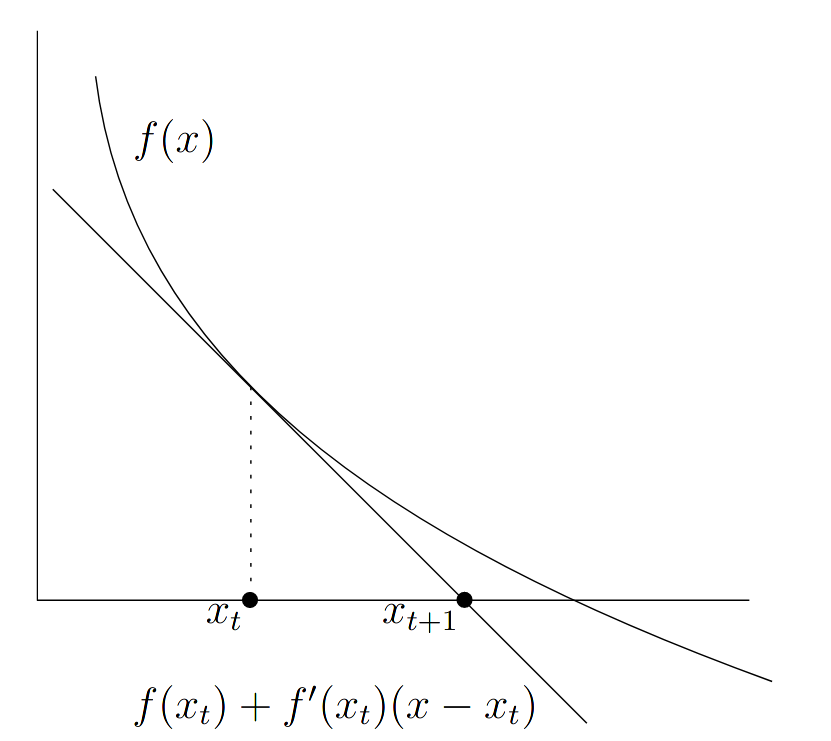
\includegraphics[width=\textwidth,height=\textheight,keepaspectratio]{newton-raphson}
      % \caption{\label{fig:label} }
    \end{figure}
  \end{minipage}
\end{frame}

\begin{frame}
  \frametitle{The Babylonian method}
  \begin{itemize}
    \item \textcolor{blue}{compute square root} of $R \in \R_+$
    \item find zero of $f(x) = x^2 - R$
    \item use Newton-Raphson:
          \begin{equation}
            x_{k+1} = x_k - \frac{f(x_k)}{f'(x_k)} = x_k - \frac{x_k^2 - R}{2 x_k} = \frac12 \left( x_k + \frac{R}{x_k} \right)
          \end{equation}
    \item Starting from $x_0 > 0$ we have
          \begin{equation}
            x_{k+1} = \frac12 \left( x_k + \frac{R}{x_k} \right) \ge \frac{x_k}{2}.
          \end{equation}
    \item Starting from $x_0 = R \ge 1$, it takes $\mathcal{O}(\log R)$ steps to get to $x_k - \sqrt{R} < \frac12$.
  \end{itemize}
\end{frame}

\begin{frame}
  \frametitle{The Babylonian method - Takeoff}
  If $x_k - \sqrt{R} < \frac12$ (ensured after $\log R$ steps).
  \begin{equation}
    x_{k+1} - \sqrt{R} = \frac12 \left( x_k + \frac{R}{x_k} \right) - \sqrt{R} = \frac{x_k}{2} + \frac{R}{2 x_k} - \sqrt{R} = \frac{1}{2 x_k} {\left( x_k - \sqrt{R} \right)}^2
  \end{equation}


\end{frame}

\end{document}
